\documentclass[12pt,letterpaper]{report}
\usepackage{pgf, tikz}
\usetikzlibrary{arrows, automata,shapes.geometric}

\begin{document}
\tikzset{elliptic state/.style={draw,ellipse}}
        \tikzstyle{every state}=[
            draw = black,
            thick,
            fill = white,
            minimum size = 20mm
        ]
    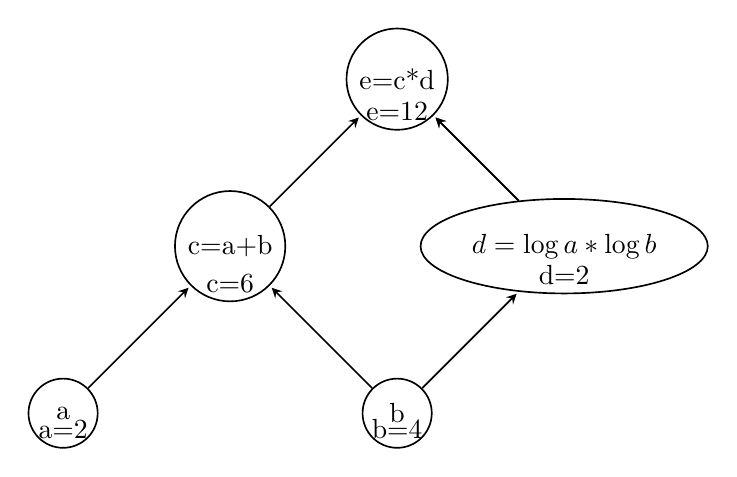
\begin{tikzpicture}[
            > = stealth, % arrow head style
            shorten > = 1pt, % don't touch arrow head to node auto,
            node distance = 3cm, % distance between nodes
            semithick, % line style
            transform shape
        ]
        

        \node[state] (e) {e=c*d};
        \node[align=center,anchor=south] (elabel) at (e.south) {e=12};

        
        \node[state] (c) [below left of=e]{c=a+b};
        \node[align=center,anchor=south] (clabel) at (c.south) {c=6};

        \node[draw,ellipse,minimum size=12mm] (d) [below right of=e]{$d=\log a*\log b$};
        \node[align=center,anchor=south] (dlabel) at (d.south) {d=2};
        
        \node[state] (a) [below left of=c]{a};
        \node[align=center,anchor=south] (alabel) at (a.south) {a=2};

        \node[state] (b) [below right of=c]{b};
        \node[align=center,anchor=south] (blabel) at (b.south) {b=4};
       
        %\node[rectangle,draw] (tmp)[above of=s]{$tmp$};
        %\node[state] (v1) [above right of=s] {$v_1$};
        %\node[state] (v2) [right of=s] {$v_2$};
        %\node[state] (v3) [below right of=s] {$v_2$};
        %\node[state] (t) [right of=v2] {$t$};
     
        \path[->] (d)  edge (e);
        \path[->]  (c) edge (e);
        \path[->] (a) edge (c);
        \path[->] (b) edge (d);
        \path[->] (d) edge (e);
        \path[->] (b) edge (c);
        


        %\path[->] (s) edge node {18} (v1);
        %\path[->] (s) edge node {1} (v2);
        %\path[->] (s) edge node {1} (v3);
        %\path[->] (v2) edge node {2} (v1);
        %\path[->] (v3) edge node {1} (v2);
        %\path[->] (v1) edge node {20} (t);

        %\draw[red, dashed] (1, 2) -- (1, -2);
    \end{tikzpicture}

\end{document}